\section{Linear parameter estimation} 
\label{LinParamEst}

As it is shown in \eqref{InputOutputmodel}, both $g(.)$ and $u(.)$ are vector-valued non-linear functions of the flow. Since the flows, the ODs and the differential pressure inputs, $dp$, are all functions of time, it can be stated that the differential equation describing the system is a first-order non-linear systems of differential equations. The number of equations are defined by the number of free variables, therefore the number of states.
\\
In this section it is shown how the model describing the network is linearized with the help of Taylor-series. Furthermore, the parameter estimation is explained. [source] 

\subsection{Taylor expansion on a simple example}
 \label{Taylorexamplesection}

The method of linearization is introduced on a simple one-state, one-input variable system. The consideration behind the example is analogous to the method applied for the water distribution system. In \eqref{example_system} the system with one state variable and one input can be seen: 

\begin{equation}
\frac{d}{dt} x = f(x,u)
 \label{example_system}
\end{equation}

Writing up $f(x,u)$ with Taylor-series the following yields: 

\begin{equation}
f(x,u) = f(\bar{x},\bar{u}) + \frac{\partial f}{\partial x}_{|\bar{x}, \bar{u}} \hat{x} + \frac{\partial f}{\partial u}_{|\bar{x}, \bar{u}} \hat{u} + higher \; order \; terms  
 \label{TaylorExpansion}
\end{equation}

\begin{minipage}[t]{0.20\textwidth}
Where\\
\hspace*{8mm} $\bar{x} \;$ and $\; \bar{u}$ \\
\hspace*{8mm} $\hat{x} \;$ and $\; \hat{u}$ 
\end{minipage}
\begin{minipage}[t]{0.68\textwidth}
\vspace*{2mm}
is the operating point ,\\
is the deviation from the operating point.
\end{minipage}

The aim of the linearization is to describe the function $f(x,u)$ around an operating point as a linear function. However, it should be noted that the approximation around this point is only valid for cases when the deviation from this point is small. Therefore the linearized version of a dynamic model is often called the small-signal model of the system. 
\\
In \eqref{TaylorExpansion}, the linearized term of $f(x,u)$ can be expressed by neglecting the affine term in the operating point, $f(\bar{x},\bar{u})$, and cancelling the higher order terms. Since the model is described by small-signals, quadratic and higher order terms result in very small values, therefore they are negligible. 
\\
The following expression in \eqref{TaylorExpansion_approx} gives the approximation of the function: 
%As it is shown in \eqref{TaylorExpansion}, the linearized version of $f$ can be expressed as the function value in the operating point, the partial derivatives of $f$ according to the input and state variable in the operating points, and the higher order versions of the partial derivatives. Since $\hat{x} = x - \bar{x}$ describe small deviations from the operating point, it is unnecessary to consider higher than first order terms. 

\begin{equation}
\frac{d}{dt} x = f(x,u) \approx \frac{\partial f}{\partial x}_{|\bar{x}, \bar{u}} (x-\bar{x}) + \frac{\partial f}{\partial u}_{|\bar{x}, \bar{u}} (u-\bar{u}) 
 \label{TaylorExpansion_approx}
\end{equation}

In case of a pipe or a valve component, the pressure drop across the element is described by a quadratic function of the flow if steady-state is considered and the dynamics are neglected. For the sake of illustration, \figref{fig:linearization} describes a non-linear function, $f(q)$, and its linearized interpretation for the operating values of pressure and flow. 

%tikz of the linearization
\begin{figure}[H]
\centering

\begin{tikzpicture} [scale=0.8,transform shape]

\usetikzlibrary{decorations.markings}

%  \draw[|-|] (5.87,-11) --
%        node[fill=white,font=\normalsize,inner ysep=2pt,inner
%                xsep=0]{$\hat{q}$}(5.5,-11);
                
% \draw[|-|] (2,-9) --
%       node[fill=white,font=\normalsize,inner ysep=2pt,inner
%               xsep=0]{$\Delta \hat{p}$}(2,-8.5);
\node at (5.2,-8.75) {$O$};
\node at (6.3,-8.5) {$O'$};
\node at (1,-4.5) {$\Delta p$};
\node at (8,-6.1) {$\Delta p = f(q)$};
\node at (8.4,-7.5) {$\Delta p = f_{linear}(q)$};
\node at (1,-9) {$\Delta \bar{p}$};
\node at (9.5,-12) {$q$};
\node at (5.5,-12) {$\bar{q}$};
\node at (8.5,-9.5) {$\hat{q}$};
\node at (5,-6) {$\Delta \hat{p}$};
\draw [->](1.5,-11.5) -- (1.5,-4.5);
\draw [->](1.5,-11.5) -- (9.5,-11.5);
\draw  plot[smooth, tension=.7] coordinates {(1.5,-11.5) (3,-10) (5.5,-9) (6.5,-7) (8,-6.5)};

\draw [black,fill=black] (5.87,-8.5) node (v4) {} circle (.35ex);
\draw [black,fill=black] (5.5,-9) node (v4) {} circle (.35ex);
\draw [thin](8,-6.5) -- (3,-11.5);
\draw [dashed](5.5,-9) -- (5.5,-11.5);
\draw [dashed](5.5,-9) -- (1.5,-9);
\draw [dashed](5.87,-8.5) -- (5.87,-11.5);
\draw [dashed](5.87,-8.5) -- (1.5,-8.5);
\draw [->](5.5,-9) -- (5.5,-6);
\draw [->](5.5,-9) -- (8.5,-9);
\end{tikzpicture} 
\caption{Linearization of a non-linear function $f(q).$}
\label{fig:linearization}
\end{figure}

As can be seen, the line inserted in the operating point, $O$, describes the model accurately only if the deviation is very small from this point, for example $O'$. Therefore the linearized model describes the system behavior in the new coordinate system $(\bar{q},\Delta \bar{p})$. It is important to mention that in \figref{fig:linearization} the function $f(q)$ is an illustration of a non-linear function and not the exact same as for a pipe element. 

%
%asdf
%
%\begin{equation}
% \hat{\Delta p} = \Delta p -  \overset{*}{\Delta p}
%\label{p_operating}
%\end{equation}
%
%asdf
%
%\begin{equation}
% \hat{z} = z -  \overset{*}{z}
%\label{p_operating}
%\end{equation}

\subsection{Linear system model}
 \label{SystemLin}
 
As it is shown in \eqref{CompleteModel_extended}, the vectorfield describing the pressure in the network consists of the pressure drops of each different elements, such as pipes$(\lambda(q) + \zeta + J \dot{q})$, valves$(\mu(q,OD))$, pumps$(\alpha(\omega, q))$, the WT $(\Delta p_{WT})$ and the WT connection $(\gamma(q))$.
\\
Among these functions, the pipes, valves, the pumps and the edge describing the WT connection are non-linear functions, therefore they need to be linearized. The linearization is carried out according to Taylor-expansion [source].
\\
The expression describing the pipes consists of three terms, one responsible for the resistances and form losses, one for the dynamics, and the last one for the elevation if there is any present. Since the elevation is not flow dependant and the dynamics are linear functions of the flow derivatives, only the model of the pipes should be linearized. 
\\
The expression describing the pipes can be approximated by its linear model as follows:

\begin{equation}
  \pmb{B_1} \lambda(\pmb{{B_1^{T}}}\pmb{z}) \approx \pmb{B_1} \bigg[ \frac{\partial{\lambda(\pmb{{B_1^{T}}}\pmb{z})}}{{\partial{\pmb{{B_1^{T}}}\pmb{z}}}}   \bigg]_{\bar{z}} \pmb{{B_1^{T}}}\pmb{\hat{z}}
\label{lambda_lin}
\end{equation}

where the partial derivative is a Jacobian matrix which is the matrix of all first-order partial derivatives of the vectorfield, $\lambda$, in the operating point $\bar{z}$. Since the derivation is according to $\pmb{{B_1^{T}}}\pmb{z}$, due to the chain rule the derivative is multiplied by $\pmb{{B_1^{T}}}$. 


In case of the valves, $\mu(\pmb{{B_1^{T}}}\pmb{z}, \pmb{OD})$ is not only the function of the independent flows, but also the opening degree. The conductivity function, $k_v$ is the function of OD, which can vary in time. Therefore the linearization has to be done according to the flow and the OD: 

\begin{equation}
  \pmb{B_1} \mu(\pmb{{B_1^{T}}}\pmb{z}, \pmb{OD}) \approx 
  \pmb{B_1} \bigg[ \frac{\partial{\mu(\pmb{{B_1^{T}}}\pmb{z}, \pmb{OD})}}{{\partial{\pmb{{B_1^{T}}}\pmb{z}}}}  \bigg]_{(\bar{z}, \bar{OD})} \pmb{{B_1^{T}}} \pmb{\hat{z}}
 +  \pmb{B_1} \bigg[ \frac{\partial{\mu(\pmb{{B_1^{T}}}\pmb{z}, \pmb{OD})}}{{\partial{\pmb{OD}}}}  \bigg]_{(\bar{z}, \bar{OD})} \pmb{{B_1^{T}}} \pmb{\hat{OD}}
\label{mu_lin}
\end{equation}

The Taylor-expansion is carried out in the same manner as in \eqref{lambda_lin}, however the linearized valve model is in the function of two small-signal variables, the flows and the OD. Therefore the partial derivatives are calculated in the operating point defined by the operating value of $\pmb{z}$ and $\pmb{OD}$. 
\\
For the water tower connection, the same can be concluded as for the pipe model. 

\begin{equation}
  \pmb{B_1} \gamma(\pmb{{B_1^{T}}}\pmb{z}) \approx \pmb{B_1} \bigg[ \frac{\partial{\gamma(\pmb{{B_1^{T}}}\pmb{z})}}{{\partial{\pmb{{B_1^{T}}}\pmb{z}}}}   \bigg]_{\bar{z}} \pmb{{B_1^{T}}}\pmb{\hat{z}}
\label{gamma_lin}
\end{equation}

The pumps are operating according to the model described in \eqref{omega_notzero}, where the valves around it are taken into account. 

\begin{equation}
\pmb{B_1} \alpha(\pmb{\omega},\pmb{z}) = \pmb{B_1} \pmb{G} \pmb{u}
\label{gamma_lin}
\end{equation}

where 

\begin{equation}
\pmb{u} =
\begin{bmatrix} 
OD_{c13} \\
OD_{c15} \\
OD_{c20} \\
OD_{c22} \\
dP_{c01} \\
dP_{c08} \\
dP_{c09} \\
dP_{c16} 
\label{inputvector}
\end{bmatrix} 
\end{equation}



For the sake of clearance, \eqref{InputOutputmodel} is shown again  

\begin{equation}
 \pmb{B}\pmb{J {B}}^T \pmb{\dot{z}} = \pmb{B} g(\pmb{B}^T \pmb{z})+ \pmb{B} u(\pmb{\omega},\pmb{k_v	}, \pmb{B}^T \pmb{z})
 \label{InputOutputmodel}
\end{equation}

asd

\begin{equation}
\Delta \dot{p}_{WT} = \frac{1}{C_H} q_0
 \label{WT_eq}
\end{equation}

asd

\begin{equation}
 \pmb{B}\pmb{J {B}}^T \pmb{\dot{z}} = \pmb{A} \pmb{\hat{z}} + \pmb{B_u} \pmb{\hat{u}} + \pmb{B_o} \Delta \hat{p}_{WT}    
 \label{statespace_1}
\end{equation}

asd

\begin{equation}
  \pmb{A}\pmb{\hat{z}} = \bigg[\pmb{B_1} \bigg[ \frac{\partial{\lambda(\pmb{{B_1^{T}}}\pmb{z})}}{{\partial{\pmb{{B_1^{T}}}\pmb{z}}}}   \bigg]_{\bar{z}} \pmb{{B_1^{T}}} +  \pmb{B_1} \bigg[ \frac{\partial{\mu(\pmb{{B_1^{T}}}\pmb{z}, \pmb{OD})}}{{\partial{\pmb{{B_1^{T}}}\pmb{z}}}}  \bigg]_{(\bar{z}, \bar{OD})} \pmb{{B_1^{T}}} +  \pmb{B_1} \bigg[ \frac{\partial{\gamma(\pmb{{B_1^{T}}}\pmb{z})}}{{\partial{\pmb{{B_1^{T}}}\pmb{z}}}}   \bigg]_{\bar{z}} \pmb{{B_1^{T}}}\bigg] \pmb{\hat{z}} 
\label{Amatrix}
\end{equation}

asd

\begin{equation}
  \pmb{B_u}\pmb{\hat{u}} = \bigg[\pmb{B_1} \bigg[ \frac{\partial{\mu(\pmb{{B_1^{T}}}\pmb{z}, \pmb{OD})}}{{\partial{\pmb{OD}}}}  \bigg]_{(\bar{z}, \bar{OD})} + \pmb{B_1}\pmb{G}\bigg] \pmb{\hat{u}} 
\label{Bumatrix}
\end{equation}

asd

\begin{equation}
 0 = \pmb{A} \pmb{\hat{z}} + \pmb{B_u} \pmb{\hat{u}} + \pmb{B_o} \Delta \hat{p}_{WT}    
 \label{statespace_2}
\end{equation}

asd

\begin{equation}
 \pmb{\hat{z}} = -(\pmb{A^{-1}}\pmb{B_u})\pmb{\hat{u}} - (\pmb{A^{-1}}\pmb{B_o})\Delta \hat{p}_{WT}    
 \label{statespace_2}
\end{equation}

asd

\begin{equation}
 \pmb{H_1}\pmb{q_1} = \pmb{H_0}q_0  
 \label{currentlaw_1}
\end{equation}

asd

\begin{equation}
q_0 = -\pmb{H^{\dagger}_0}\pmb{H_1}\pmb{q_1}
 \label{currentlaw_2}
\end{equation}

asd

\begin{equation}
\Delta \dot{p}_{WT} = - \frac{1}{C_H} \pmb{H^{\dagger}_0}\pmb{H_1}\pmb{q_1} = - \underbrace{\frac{1}{C_H} \pmb{H^+_0}\pmb{H_1}\pmb{{B_1^{T}}}}_\text{\pmb{H}} z
 \label{currentlaw_2}
\end{equation}

\begin{equation}
\Delta \dot{p}_{WT} = \underbrace{(\pmb{H}\pmb{A^{-1}}\pmb{B_o})}_\text{\pmb{M}}\Delta \hat{p}_{WT}  + \underbrace{(\pmb{H}\pmb{A^{-1}}\pmb{B_u})}_\text{\pmb{N}}\pmb{\hat{u}}  
 \label{statespace_3}
\end{equation}

\begin{equation}
\Delta \dot{p}_{WT} = \pmb{M} \Delta \hat{p}_{WT}  + \pmb{N}\pmb{\hat{u}}  
 \label{statespace_4}
\end{equation}

\begin{equation}
\pmb{y} = \pmb{C} \Delta \hat{p}_{WT}  + \pmb{D}\pmb{\hat{u}}  
 \label{statespace_5}
\end{equation}

%Using the same logic as for the one state-one input system, it can be assumed that the system dynamics in the proximity of the operating point trajectories can be approximated by the first terms of Taylor series. Since the system dynamics consist of time dependant non-linear vectorfields, the system model can be considered as: 
%
%\begin{equation}
%\frac{d}{dt} \pmb{x(t)} = \mathcal{F}(\pmb{x(t)},\pmb{u(t)})
% \label{sysfunc_simplified}
%\end{equation}
%
%Where the state and input expressions are considered as: 
%
%\begin{equation}
%\pmb{x(t)} = \pmb{\bar{x(t)}} + \pmb{\hat{x(t)}}
% \label{gfunc}
%\end{equation}
%
%and 
%
%\begin{equation}
%\pmb{u(t)} = \pmb{\bar{u(t)}} + \pmb{\hat{u(t)}}
% \label{ufunc}
%\end{equation}
%
%\eqref{sysfunc_simplified} is in the same form as the original system model, therefore for the sake of simplicity, it is used to show how the linearization of such a model is carried out. 
%\\
%By expanding the right-hand side into the Taylor series, using \eqref{gfunc} and \eqref{ufunc}, the following yields:
%
%\begin{equation}
%\frac{d}{dt} (\pmb{\bar{x}} + \pmb{\hat{x}})  \approx \mathcal{F}(\pmb{\bar{x}(t)} + \pmb{\hat{x}(t)}, \pmb{\bar{u}(t)} + \pmb{\hat{u}(t)} )
% = \mathcal{F}(\pmb{\bar{x}},\pmb{\bar{u}}) + \frac{\partial {\mathcal{F}}}{\partial \pmb{x}}_{|\bar{x}, \bar{u}} \pmb{\hat{x}} + \frac{\partial {\mathcal{F}}}{\partial \pmb{u}}_{|\bar{x}, \bar{u}} \pmb{\hat{u}} 
% \label{multistate model_full}
%\end{equation}
%
%Thus the small signal model of such a multi-state model can be expressed as: 
%
%\begin{equation}
%\frac{d}{dt} \pmb{\hat{x}}  \approx
% = \frac{\partial {\mathcal{F}}}{\partial \pmb{x}}_{|\bar{x}, \bar{u}} \pmb{\hat{x}} + \frac{\partial {\mathcal{F}}}{\partial \pmb{u}}_{|\bar{x}, \bar{u}} \pmb{\hat{u}} 
% \label{multistate model_smallsignal}
%\end{equation}
%
%%\begin{equation}
%%\frac{d}{dt} \pmb{\bar{x}} + \frac{d}{dt} \pmb{\hat{x}}  \approx \mathcal{F}(\pmb{\bar{x(t)}} + \pmb{\hat{x(t)}}, \pmb{\bar{u(t)}} + \pmb{\hat{u(t)}} )
%% = \mathcal{F}(\pmb{\bar{x}},\pmb{\bar{u}}) 
%%
%%\label{TaylorExpansion_approx}
%%\end{equation}

As can be seen in \eqref{multistate model_smallsignal}, the small signal model of such a multi-state/ multi-input system consists of two Jacobian matrices, one for the states and one for the inputs to the system. It should be emphasized however that these matrices have to be evaluated at the operating points, at $(\bar{x}, \bar{u})$. It is a reasonable statement since the inputs to the model are the small signal values of OD and differential pressures, dp, from the pumps. Therefore the same excitation to the real test setup can be carried out by taking the operating values into account and by adding them to the small signal values. 

\begin{figure}[H]
\centering
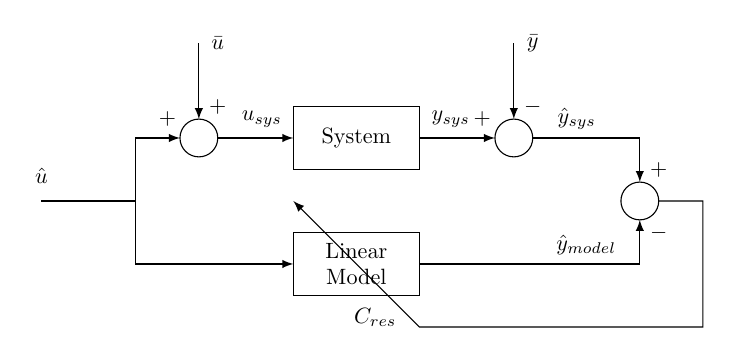
\begin{tikzpicture} [scale=0.8,transform shape]

\draw  (3,-1.5) rectangle (5,-2.5);
\node at (4,-1.8) {Linear};
\node at (4,-2.2) {Model};

\draw  (3,0.5) rectangle (5,-0.5);
\node at (4,0) {System};

\node at (8.8,-1.5) {$-$};
\node at (5.5,0.3) {$y_{sys}$};
\node at (7.5,0.3) {$\hat{y}_{sys}$};
\node at (7.65,-1.7) {$\hat{y}_{model}$};
\node at (4.3,-2.85) {$C_{res}$};
\node at (-1,-0.6) {$\hat{u}$};
\node at (1.8,1.5) {$\bar{u}$};
\node at (2.5,0.3) {$u_{sys}$};
\node at (8.8,-0.5) {$+$};
\node at (1.8,0.5) {$+$};
\node at (6,0.3) {$+$};
\node at (6.8,0.5) {$-$};
\node at (1,0.3) {$+$};
\node at (6.8,1.5) {$\bar{y}$};

\draw  (8.5,-1) ellipse (0.3 and 0.3);
\draw  (6.5,0) ellipse (0.3 and 0.3);
\draw  (1.5,0) ellipse (0.3 and 0.3);

\draw [-latex](5,0) -- (6.2,0);

\draw [-latex](0.5,-1) -- (0.5,0) -- (1.2,0);
\draw [-latex](0.5,-1) -- (0.5,-2) -- (3,-2);
\draw (-1,-1) -- (0.5,-1);
\draw [-latex](5,-2) -- (8.5,-2) -- (8.5,-1.3);
\draw [-latex](8.8,-1) -- (9.5,-1) -- (9.5,-3) -- (5,-3) -- (3,-1);

\draw [-latex](1.8,0) -- (3,0);
\draw [-latex](1.5,1.5) -- (1.5,0.3);
\draw [-latex](6.5,1.5) -- (6.5,0.3);
\draw [-latex](6.8,0) -- (8.5,0) -- (8.5,-0.7);
\end{tikzpicture}% 
\caption{Parameter identification block diagram for the linear system. }
\label{fig:parame_block_lin}
\end{figure}

%Note: 
%After this, the general structure of the matrices and the same formulation for the water distribution system will be written. 
%
%The linearization procedure of both $g(\pmb{q})$ and $u(\pmb{\omega},\pmb{OD}, \pmb{B^T z})$, is shown:
%
%\begin{equation}
%  \begin{split}
%  & B g_{i}({B_{1}}^{T}z) = B_1 \frac{\partial{\lambda_{i}({{B_{1}}^{T}z})}}{\partial{B_{1}^{T}z}} {B_1}^{T} \quad + \quad
%  B_0 {\hat{\Delta P}}_{WT} \quad + \quad B_1 \frac{\partial{\mu_{i}({{B_{1}}^{T}z})}}{\partial{B_{1}^{T}z}} {B_1}^{T} \quad - \\
%  &  B_0 \alpha_{i}(B_{1}^{T}z) \quad + \quad B_0 \frac{\partial{\mu_{i}({{B_{0}}^{T}z})}}{\partial{B_{0}^{T}z}} {B_0}^{T}
%  \end{split}
%  \label{StateLinear}
%\end{equation}
%
%\begin{equation}
%  B \mu_{i}(\omega, OD, {B_1}^{T}z) = - B_1 \alpha_{i}(dP) \quad + \quad B_1 \frac{\partial{\mu_{i}(OD)}}{\partial{OD}} {B_1}^{T}
%  \quad + \quad B_0 \frac{\partial{\mu_{i}(OD)}}{\partial{OD}} {B_0}^{T}
%  \label{inputlinear}
%\end{equation}
%
%
%
%These expressions below are for the following documentation, there are not any explanation for them yet. We did not comment them out because some parts might be useful to look at
%
%
%\begin{equation}
% \dot{\Delta p_{WT}} = \frac{1}{C_H} q_{WT}
%\label{WTeq1}
%\end{equation}
%
%\begin{equation}
% \pmb{ \Delta p} = \pmb{J \dot{q_1}} + \lambda(\pmb{q_1}) + \zeta + \mu(\pmb{q_1}, \pmb{OD}) - \alpha(\pmb{dp})
%\label{NonlinearPressureFunction}
%\end{equation}
%
%asdf
%
%\begin{equation}
% \dot{\Delta p_{WT}} = \frac{1}{C_H} q_{WT}
%\label{WTeq2}
%\end{equation}
%
%asdf
%
%\begin{equation}
%\pmb{\Delta p_0} =
%\begin{bmatrix}
%         \Delta p_{C32} \\
%	\Delta p_{WT}
%\end{bmatrix}
%\label{pvector}
%\end{equation}
%
%asdf
%
%\begin{equation}
%\pmb{q_0} =
%\begin{bmatrix}
%         q_{C32} \\
%	q_{WT}
%\end{bmatrix}
%\label{qvector}
%\end{equation}
%
%Recalling \eqref{InputOutputmodel_steadystate}:
%
%\begin{equation}
% \pmb{B}\pmb{J} \pmb{\dot{q}} = \pmb{B} g(\pmb{q})+ \pmb{B_1} u(\pmb{\omega},\pmb{OD})
% \label{InputOutputmodel_steadystate_linmodel}
%\end{equation}
%
%\begin{equation}
%\label{gfunction}
% g_{i}(q) =
%		\left\{
%		\begin{array}{ll}
%		
%		\lambda_i(q_1) 			&      \text{for i = ...}	
%\\
%		\lambda_i(q_1) + \zeta_i                      &     \text{for i = ...}
%\\
%
%                \Delta p_{WT;i}                       &      \text{for i = ...}
%\\
%
%                \mu_{i;q1}(q_1, OD)                       &      \text{for i = ...}
%
%		\end{array}
%		\right.
%\end{equation}	
%
%\begin{equation}
%\label{ufunction}
% u_{i}(\omega, OD) =
%		\left\{
%		\begin{array}{ll}
%		
%		\alpha_i(\omega) 			&      \text{for i = ...}	
%\\
%		\mu_{i;OD}(q_1, OD)                      &     \text{for i = ...}
%
%		\end{array}
%		\right.
%\end{equation}	





\subsection{Linear Model Implementation}
\label{MatlabScriptLinear}

Unlike for the nonlinear model, in the linear model the WT is taken into consideration. Therefore, the state vector is augmented into a $9x1$ vector, 
containing the 8 chord flows and the pressure across the WT. For the linear model a state-space system is designed.

The state matrix, $A$, is conformed by the linearized friction provided by the pipes, the linearized part of the valve function corresponding to the state and pressure contribution
of the WT.

Pipes contribution:

\begin{equation}
  {\lambda}_e = (2 * Cp * {B_1}^{T} \, abs(\hat{z}) /(10^5*3600^2))
  \label{lambdafun}
\end{equation}

\eqref{lambdafun} only affects to the 8 chords of the water distribution, lambda ends up being a $25x1$ matrix. However, we will have a lambda expression for all pipes
edges, resulting in a $25x25$ adding $0$ for those non-pipe edges. 

Valve contribution:

\vspace{4mm}
\begin{equation}
  {\mu}_e = e^{\frac{2 \, (\theta_{off} - \bar{OD}) \, n_{gl}}{\theta_{max}-\theta_{off}}+2} \, \bar{z} \, |\bar{z}| \quad \quad - \\
  2 \, e^{\frac{2 \, (\theta_{off} - \bar{OD}) \, n_{gl}}{\theta_{max}-\theta_{off}}+2} \, {B_1}^{T} abs(\hat{z}) \, |\bar{z}|
  \label{mufun}
\end{equation}

The above expression has been derived in \appref{chap:Lin}, for the state matrix only the part corresponding to the states is taken. In the same way 
as in the pipe, the $\mu$ expression for each edge is a $25x1$ matrix. This extended to all the edges will end up into a $25x25$ matrix, with $0$ in the 
non-valve edges. 

When augmenting the system with the WT, two new edges show up in the water distribution. This two new edges are the WT itself and a pump connected to the WT.
The pump connected to the WT is running with $0$ rotational speed, thus the mathematical model results in:

\begin{equation}
    \Delta p = -a_{h2}{q_i}^2 
\end{equation}

Along with the pump there are two pumps, gathering all the components expressions:

\begin{equation}
      \Delta p = (\frac{2}{{k_v}^2-a_{h2}}){q_i}^2 
\end{equation} \todo{Add the linearization explanation into the Appendix}

The above equation needs to be linearized and consequently separate into the state and the input part. The contribution to the $A$ matrix is as 
following:

\begin{equation}
  \alpha = 2 * e^{\frac{2 \, (\theta_{off} - \bar{OD}) \, n_{gl}}{\theta_{max}-\theta_{off}}+2} \, \bar{z} \, |\bar{z}| \quad - \\
  4 \, e^{\frac{2 \, (\theta_{off} - \bar{OD}) \, n_{gl}}{\theta_{max}-\theta_{off}}+2} \, {B_0}^{T} abs(\hat{z}) \, |\bar{z}| - 2 * {B_0}^{T} abs(\hat{z}) * c.Ah22
\end{equation}

The cycle matrix, $B_0$ corresponding to the augmented system is used with dimensions $8x2$ but the state vector of the 8 flow chords.
 The $\alpha$ function results in a $2x2$ matrix with $0$ in the column corresponding to the non-pump edge. 

In regards to the WT edge, the pressure across it is treated as a new state for the system, that is, the ninth state $\Delta p_{WT}$. 

Once the terms conforming the $A$ matrix are identified, the correct structure due to the linearization has to be applied as explained in \secref{} resulting in
the following $A$ matrix.

\begin{equation}
  A = B_1 \, \lambda \, {B_1}^T + B_1 \, \mu \, {B_1}^T + B_0 \, \alpha \, {B_0}^T
\end{equation}

The remain $A$ matriz has the dimension $8x8$ and the new state $\Delta p_{WT}$ of the WT has to be included into the matrix in order to get an $9x9$ $A$ 
matrix. 

The input matrix, $B$, is conformed by the input into the system. These are the opening degree of the valves and the pressure contribution of the main 
and PMA pumps. 

Previously, for the $A$ matrix the valve expression has been linearized, this time the input term of the linearized expression will be taken:

\begin{equation}
  {\mu}_e = -2 \, \frac{e^{\frac{2 \, (\theta_{off} - \bar{OD}) \, n_{gl}}{\theta_{max}-\theta_{off}}+2}
   \, n_{gl} \, \hat{OD} \, \bar{q} \, |\bar{q}|}{\theta_{max}-\theta_{off}}
\end{equation}

The pumps pressure contribution is also added into the input matrix. 


